% Part: sets-functions-relations
% Chapter: relations
% Section: trees

\documentclass[../../../include/open-logic-section]{subfiles}

\begin{document}

\olfileid{sfr}{rel}{tre}
\olsection{Bomen}

Een \emph{boom} is een bepaald soort partiële ordening. Zulke bomen
spelen in elk deel van de logica een belangrijke rol. In de
eenvoudigere delen van de logica kom je eindige bomen tegen. Zo kun je
!!{formula}s begrijpen door te kijken hoe ze in een syntaxisboom in
kleinere delen uiteenvallen. Ook !!{derivation}s hebben in veel
systemen voor !!{derivation}s de vorm van een eindige boom.
%
Oneindige bomen kom je al tegen in het bewijs van de
volledigheidsstellingen voor propositielogica en eerste-ordelogica. Ze
worden in de hele wiskundige logica gebruikt.

Wat in de verzamelingenleer een boom heet, lijkt sterk op een boom uit
de grafentheorie. Zo ziet een (eindige) boom eruit:

\begin{center}
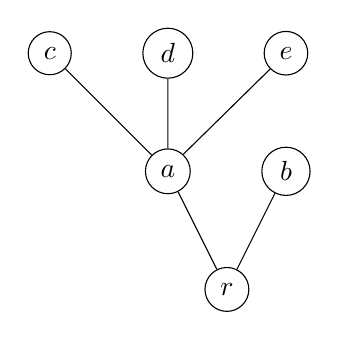
\begin{tikzpicture}[nodes={draw, circle}, -]
\node{$r$} [grow'=up]
    child { node {$a$} 
        child { node {$c$} }
        child { node {$d$} }
        child { node {$e$} }
    }
    child { node {$b$} };
\end{tikzpicture}
\end{center}

De onderste knoop~$r$ heet de wortel. Elke knoop behalve $r$ heeft
vlak eronder precies één ouder. Neem twee knopen~$x$ en~$y$. Kun je
$y$ vanuit~$x$ bereiken door de lijnen omhoog te volgen, dan heet $x$
een \emph{voorouder} van~$y$.

De voorouderrelatie van een boom is een strikte partiële ordening.
Daarom gebruiken we die relatie in de definitie met verzamelingen.
Eerst moeten we twee begrippen uitleggen. Een \emph{kleinste element}
in een verzameling~$A$ die partieel is geordend door~$\le$, is
!!a{element} $x \in A$ waarvoor bij elk $y \in A$ geldt dat~$x \le y$.
We noemen een verzameling door~$\le$ \emph{welgeordend} als elke
deelverzameling waar iets in zit een kleinste element heeft.

\begin{defn}[Boom]
Een \emph{boom} is een paar $T = \tuple{A, \le}$. Hier is $A$ een
verzameling en is $\le$ een partiële ordening op~$A$. Deze ordening
heeft precies één kleinste element $r \in A$ (de \emph{wortel}).
Verder is voor elk $x \in A$ de verzameling
$\Setabs{y}{y \le x}$ welgeordend door~$\le$.
\end{defn}

\begin{defn}[Opvolgers]
Neem een boom $T = \tuple{A, \le}$.
Als $x,y \in A$ en $x < y$, maar er geen $z \in A$ is met
$x < z < y$, dan heet $y$ een \emph{opvolger} van~$x$.
\end{defn}

De opvolgers van $x \in A$ heten ook zijn \emph{kinderen}. Is $y$ een
opvolger van~$x$, dan heet $x$ de \emph{voorganger} of \emph{ouder}
van~$y$.

\begin{prop}
Als $\tuple{A,\le}$ een boom is, kan elk $x \in A$ dat niet de wortel
is hoogstens één voorganger hebben.
\end{prop}

\begin{proof}
  Neem aan dat $y_1 < x$ en $y_2 < x$ en dat $y_1 \neq y_2$. Dan
  geldt $\{y_1, y_2\} \subseteq \Setabs{z}{z<x}$. De verzameling
  $\Setabs{z}{z<x}$ is welgeordend door~$\le$. Daarom heeft de
  deelverzameling $\{y_1, y_2\}$ een kleinste element. Dat moet $y_1$
  of~$y_2$ zijn. Dus $y_1 \le y_2$ of $y_2 \le y_1$. We hebben
  aangenomen dat $y_1 \neq y_2$, dus eigenlijk geldt $y_1 < y_2$ of
  $y_2 < y_1$. We weten ook dat $y_1 < x$ en $y_2 < x$. Daardoor
  geldt bovendien $y_1 < y_2 < x$ of $y_2 < y_1 < x$. De elementen
  $y_1$ en $y_2$ kunnen dus niet allebei voorgangers van~$x$ zijn.
\end{proof}

\begin{defn}
Een boom $T = \tuple{A, \le}$ noemen we \emph{oneindig} als $A$ een
oneindige verzameling is, en anders \emph{eindig}. Heeft $T$ de
eigenschap dat elke $x \in A$ maar eindig veel opvolgers heeft, dan
noemen we $T$ \emph{eindig vertakkend}.
\end{defn}

\begin{defn}[Takken]
Neem een boom $T = \tuple{A, \le}$. Een \emph{tak} van~$T$ is een
maximale keten in~$T$. Dat betekent hier dat $B \subseteq A$ en dat
voor elk tweetal $x, y \in B$ geldt dat $x \le y$ of $y \le x$.
Verder bestaat voor elke $z \in A \setminus B$ een $u \in B$ waarvoor
noch $z \le u$ noch $u \le z$ geldt.
%
We schrijven $[T]$ voor de verzameling van alle takken van $T$.
\end{defn}

\begin{ex}
Een bekend voorbeeld van een eindig vertakkende boom is de
\emph{oneindige binaire boom}. Die bestaat uit alle eindige rijen
van $0$'en en~$1$'en. We schrijven deze boom soms als $\{0,1\}^*$ of
als~$\Bin^*$. De uitbreidingsrelatie $\sqsubseteq$ bepaalt hun
volgorde. Zo geldt $101 \sqsubseteq 101101$: je krijgt de tweede rij
door achter de eerste nog cijfers te zetten. Achter elke binaire rij
kun je altijd een
$0$ of een $1$ zetten. Daarom heeft deze boom oneindig veel
elementen: bij elk element~$s$ horen precies twee opvolgers, $s0$
en~$s1$. De wortel is de lege rij $\emptyseq$.
\end{ex}

\begin{ex}
Iets algemener kun je eindige rijen van natuurlijke getallen nemen.
De verzameling daarvan,~$\Nat^*$, is met de
uitbreidingsrelatie~$\sqsubseteq$ ook een boom. Deze boom is duidelijk
niet eindig vertakkend: elke $s \in \Nat^*$ heeft oneindig veel
opvolgers~$sn$, één voor elke $n \in \Nat$. Elke
$A \subseteq \Nat^*$ die onder~$\sqsubseteq$ gesloten is, is een
\emph{deelboom} van~$\Nat^*$. (Dat betekent: $A$ is zo dat uit
$s \in A$ en $s' \sqsubseteq s$ ook $s' \in A$ volgt.) Elke eindige
boom kan worden voorgesteld als een eindige deelboom van~$\Nat^*$.
\end{ex}

\begin{prop}[Lemma van K\H{o}nig]
Als $T = \tuple{A,\le}$ een oneindige boom is die eindig vertakt, dan
heeft $T$ een oneindige tak.
\end{prop}

In de berekenbaarheidstheorie, de theorie van wat berekenbaar is, wordt
vaak een speciaal geval van het lemma van K\H{o}nig gebruikt. Het heet
het \emph{zwakke lemma van
K\H{o}nig} en zegt: elke oneindige deelboom van $\{0,1\}^*$ heeft een
oneindige tak.
\end{document}
